% Options for packages loaded elsewhere
\PassOptionsToPackage{unicode}{hyperref}
\PassOptionsToPackage{hyphens}{url}
%
\documentclass[
]{book}
\usepackage{amsmath,amssymb}
\usepackage{lmodern}
\usepackage{iftex}
\ifPDFTeX
  \usepackage[T1]{fontenc}
  \usepackage[utf8]{inputenc}
  \usepackage{textcomp} % provide euro and other symbols
\else % if luatex or xetex
  \usepackage{unicode-math}
  \defaultfontfeatures{Scale=MatchLowercase}
  \defaultfontfeatures[\rmfamily]{Ligatures=TeX,Scale=1}
\fi
% Use upquote if available, for straight quotes in verbatim environments
\IfFileExists{upquote.sty}{\usepackage{upquote}}{}
\IfFileExists{microtype.sty}{% use microtype if available
  \usepackage[]{microtype}
  \UseMicrotypeSet[protrusion]{basicmath} % disable protrusion for tt fonts
}{}
\makeatletter
\@ifundefined{KOMAClassName}{% if non-KOMA class
  \IfFileExists{parskip.sty}{%
    \usepackage{parskip}
  }{% else
    \setlength{\parindent}{0pt}
    \setlength{\parskip}{6pt plus 2pt minus 1pt}}
}{% if KOMA class
  \KOMAoptions{parskip=half}}
\makeatother
\usepackage{xcolor}
\usepackage{color}
\usepackage{fancyvrb}
\newcommand{\VerbBar}{|}
\newcommand{\VERB}{\Verb[commandchars=\\\{\}]}
\DefineVerbatimEnvironment{Highlighting}{Verbatim}{commandchars=\\\{\}}
% Add ',fontsize=\small' for more characters per line
\usepackage{framed}
\definecolor{shadecolor}{RGB}{248,248,248}
\newenvironment{Shaded}{\begin{snugshade}}{\end{snugshade}}
\newcommand{\AlertTok}[1]{\textcolor[rgb]{0.94,0.16,0.16}{#1}}
\newcommand{\AnnotationTok}[1]{\textcolor[rgb]{0.56,0.35,0.01}{\textbf{\textit{#1}}}}
\newcommand{\AttributeTok}[1]{\textcolor[rgb]{0.77,0.63,0.00}{#1}}
\newcommand{\BaseNTok}[1]{\textcolor[rgb]{0.00,0.00,0.81}{#1}}
\newcommand{\BuiltInTok}[1]{#1}
\newcommand{\CharTok}[1]{\textcolor[rgb]{0.31,0.60,0.02}{#1}}
\newcommand{\CommentTok}[1]{\textcolor[rgb]{0.56,0.35,0.01}{\textit{#1}}}
\newcommand{\CommentVarTok}[1]{\textcolor[rgb]{0.56,0.35,0.01}{\textbf{\textit{#1}}}}
\newcommand{\ConstantTok}[1]{\textcolor[rgb]{0.00,0.00,0.00}{#1}}
\newcommand{\ControlFlowTok}[1]{\textcolor[rgb]{0.13,0.29,0.53}{\textbf{#1}}}
\newcommand{\DataTypeTok}[1]{\textcolor[rgb]{0.13,0.29,0.53}{#1}}
\newcommand{\DecValTok}[1]{\textcolor[rgb]{0.00,0.00,0.81}{#1}}
\newcommand{\DocumentationTok}[1]{\textcolor[rgb]{0.56,0.35,0.01}{\textbf{\textit{#1}}}}
\newcommand{\ErrorTok}[1]{\textcolor[rgb]{0.64,0.00,0.00}{\textbf{#1}}}
\newcommand{\ExtensionTok}[1]{#1}
\newcommand{\FloatTok}[1]{\textcolor[rgb]{0.00,0.00,0.81}{#1}}
\newcommand{\FunctionTok}[1]{\textcolor[rgb]{0.00,0.00,0.00}{#1}}
\newcommand{\ImportTok}[1]{#1}
\newcommand{\InformationTok}[1]{\textcolor[rgb]{0.56,0.35,0.01}{\textbf{\textit{#1}}}}
\newcommand{\KeywordTok}[1]{\textcolor[rgb]{0.13,0.29,0.53}{\textbf{#1}}}
\newcommand{\NormalTok}[1]{#1}
\newcommand{\OperatorTok}[1]{\textcolor[rgb]{0.81,0.36,0.00}{\textbf{#1}}}
\newcommand{\OtherTok}[1]{\textcolor[rgb]{0.56,0.35,0.01}{#1}}
\newcommand{\PreprocessorTok}[1]{\textcolor[rgb]{0.56,0.35,0.01}{\textit{#1}}}
\newcommand{\RegionMarkerTok}[1]{#1}
\newcommand{\SpecialCharTok}[1]{\textcolor[rgb]{0.00,0.00,0.00}{#1}}
\newcommand{\SpecialStringTok}[1]{\textcolor[rgb]{0.31,0.60,0.02}{#1}}
\newcommand{\StringTok}[1]{\textcolor[rgb]{0.31,0.60,0.02}{#1}}
\newcommand{\VariableTok}[1]{\textcolor[rgb]{0.00,0.00,0.00}{#1}}
\newcommand{\VerbatimStringTok}[1]{\textcolor[rgb]{0.31,0.60,0.02}{#1}}
\newcommand{\WarningTok}[1]{\textcolor[rgb]{0.56,0.35,0.01}{\textbf{\textit{#1}}}}
\usepackage{longtable,booktabs,array}
\usepackage{calc} % for calculating minipage widths
% Correct order of tables after \paragraph or \subparagraph
\usepackage{etoolbox}
\makeatletter
\patchcmd\longtable{\par}{\if@noskipsec\mbox{}\fi\par}{}{}
\makeatother
% Allow footnotes in longtable head/foot
\IfFileExists{footnotehyper.sty}{\usepackage{footnotehyper}}{\usepackage{footnote}}
\makesavenoteenv{longtable}
\usepackage{graphicx}
\makeatletter
\def\maxwidth{\ifdim\Gin@nat@width>\linewidth\linewidth\else\Gin@nat@width\fi}
\def\maxheight{\ifdim\Gin@nat@height>\textheight\textheight\else\Gin@nat@height\fi}
\makeatother
% Scale images if necessary, so that they will not overflow the page
% margins by default, and it is still possible to overwrite the defaults
% using explicit options in \includegraphics[width, height, ...]{}
\setkeys{Gin}{width=\maxwidth,height=\maxheight,keepaspectratio}
% Set default figure placement to htbp
\makeatletter
\def\fps@figure{htbp}
\makeatother
\setlength{\emergencystretch}{3em} % prevent overfull lines
\providecommand{\tightlist}{%
  \setlength{\itemsep}{0pt}\setlength{\parskip}{0pt}}
\setcounter{secnumdepth}{5}
\usepackage{booktabs}
\usepackage{amsthm}
\makeatletter
\def\thm@space@setup{%
  \thm@preskip=8pt plus 2pt minus 4pt
  \thm@postskip=\thm@preskip
}
\makeatother
\ifLuaTeX
  \usepackage{selnolig}  % disable illegal ligatures
\fi
\usepackage[]{natbib}
\bibliographystyle{plainnat}
\IfFileExists{bookmark.sty}{\usepackage{bookmark}}{\usepackage{hyperref}}
\IfFileExists{xurl.sty}{\usepackage{xurl}}{} % add URL line breaks if available
\urlstyle{same} % disable monospaced font for URLs
\hypersetup{
  pdftitle={An Introduction to Experimental Design ANOVA and ANCOVA},
  pdfauthor={Andrew P Beckerman (with support from text and slides from Mark Rees and Gareth Phoenix)},
  hidelinks,
  pdfcreator={LaTeX via pandoc}}

\title{An Introduction to Experimental Design ANOVA and ANCOVA}
\author{Andrew P Beckerman (with support from text and slides from Mark Rees and Gareth Phoenix)}
\date{2022-11-25}

\begin{document}
\maketitle

{
\setcounter{tocdepth}{1}
\tableofcontents
}
\hypertarget{introduction}{%
\chapter{Introduction}\label{introduction}}

Welcome to An Introduction to Experimental Design ANOVA and ANCOVA

In this mini-module, you'll be learning about the principles of experimental design and analysis of a few classic designes, the 2x2 ANOVA and ANCOVA experiments.

This module is compulsory for all, because it forms the foundation for most of the more complex experiments you will do as a researcher. And it is the major step beyond the t-test, 1-way ANOVA, simple regression and chi-square contingency table analyses we've covered thus far.

The learning outcome for this mini-module are that you will understand the basic ideas about

\begin{itemize}
\tightlist
\item
  Replication, Randomisation and Reducing Noise
\item
  Precision, Bias and Systematic Error
\item
  The Completely Randomised Design
\item
  The Randomised Block Design
\item
  The 2-way ANOVA
\item
  The ANCOVA Design
\end{itemize}

In order to be successful with this final section of the course, you need to feel comfortable with the 1-way ANOVA and the Regression model. Please review these concepts. You can also refer to Chapter 5 and 6 in Getting Started with R (available as an online Resource via STARPlus) which covers a great deal of the mechanics of using R to do these types of models. Finally, you will also need to feel comfortable with dplyr and ggplot - we'll be reinforcing the old stuff and introducing a few new tricks.

\hypertarget{the-three-rs-the-foundation-of-experimental-design.}{%
\section{The Three Rs: The Foundation of Experimental Design.}\label{the-three-rs-the-foundation-of-experimental-design.}}

Before we get started, it's vital that you understand that there are some very basic principles needed to ensure that your experiments can provide robust and reliable inference (answers to your questions). The ``3 R's''.

\begin{itemize}
\tightlist
\item
  \textbf{Randomisation}: the random allocation of treatments to the experimental units, to avoid confounding between treatment effects and other unknown effects.
\item
  \textbf{Replication}: the repetition of a treatment within an experiment, to quantify the natural variation between experimental units and increase accuracy of estimated effects.
\item
  \textbf{Reduce noise:} by controlling as much as possible the conditions in the experiment, e.g.~by grouping of similar experimental units in blocks.
\end{itemize}

As we develop our understanding of experimental design, you should come back to these core definitions and see if your understanding of them has improved. We work on these concepts in the next chapter of the book.

\hypertarget{the-general-linear-model}{%
\section{The General Linear Model}\label{the-general-linear-model}}

This section of the course is focused on a class of model called the General Linear Model. It is not a \textbf{GLM}. The \textbf{GLM} is a generalised linear model. I know, right?

The general linear model is, as we learned in the past few weeks, a model fit in R with the \texttt{lm()} function. It includes regression, ANOVA, ANCOVA and variations of these.

There are a few key characterstics to remember about these models. The general linear model has the following form:

\(y = \beta_{0}+\beta_{1}*X_{1}+\beta_{2}*X_{2}+\epsilon\)

Where the \(y\) is the response variable, the \(\beta\)'s are estimated parameters, the \(X\)'s are the predictor variables and the \(\epsilon\) comes from a Gaussian distribution with zero mean and constant variance.

Let's decompose that a bit more.

There are two types of predictor variable:

\emph{Metric} predictor variables are measurements of some quantity that may help to predict the value of the response. For example, if the response is the blood pressure of patients in a clinical trial, then age, fat mass and height are potential metric predictor variables. You may know these as \textbf{continuous explanatory (independent) variables}

\emph{Factor} variables are labels that serve to categorize the response measurements into groups, which may have different expected values. Continuing the blood pressure example, factor variables might be sex and drug treatment received (drug A, drug B or placebo, for example). You may also know these as \textbf{categorical explanatory (independent) variables}.

So, you hopefully can see how this \emph{general} linear model is capable of representing

\begin{enumerate}
\def\labelenumi{\arabic{enumi}.}
\tightlist
\item
  \emph{ANOVA} -- Analysis of variance -\textgreater{} Predictors are factors.
\item
  \emph{Regression} -\textgreater{} Predictor is a metric variable (continuous variable).\\
\item
  \emph{Multiple regression} -\textgreater{} Predictors are metric variables (continuous variables).
\item
  \emph{ANCOVA} - Analysis of co-variance -\textgreater{} Predictors are a mixture of metric variables (continuous variables) and factors.
\end{enumerate}

Finally, it is important to understand that non-linear relationships such as these data below can be modelled with a linear model:

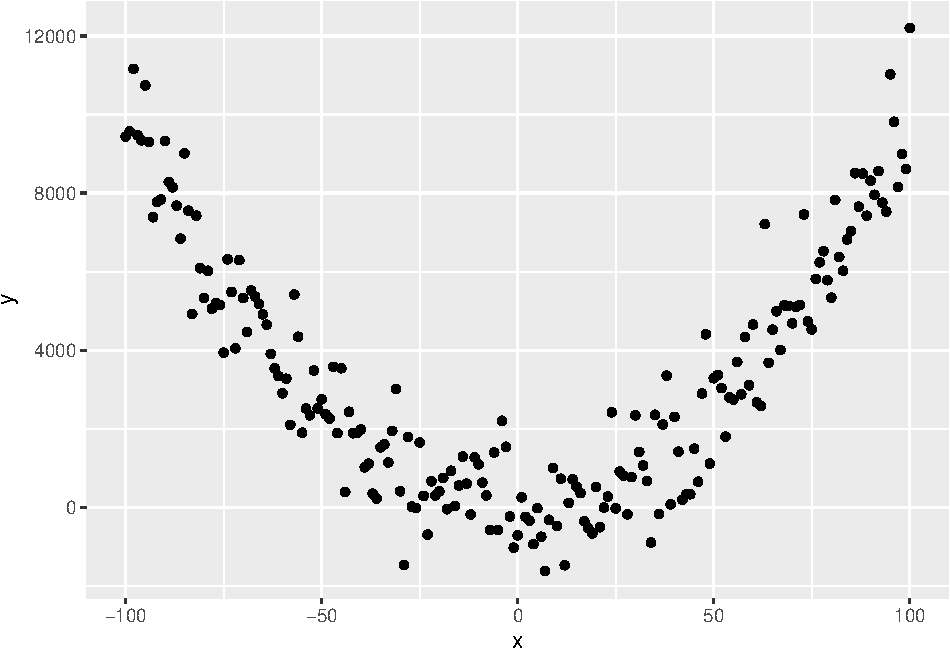
\includegraphics{bookdown-demo_files/figure-latex/unnamed-chunk-2-1.pdf}

How, you ask!? Well\ldots. consider this equation:

\(y = 0.01 + x + x^{2} + \epsilon\)

Referring to our generic model structure above,

\(y = \beta_{0}+\beta_{1}*X_{1}+\beta_{2}*X_{2}+\epsilon\)

we hopefully can see that \(\beta_{0} = 0.01\), \(\beta_{1} = 0\) and \(\beta_{2} = 1\), where \(X_{2} = X^{2}\)!

Linear models are perfectly capable of being used to estimate non-linear relationships!

Here is the code to make that figure.

\begin{Shaded}
\begin{Highlighting}[]
\CommentTok{\# set x range}
\NormalTok{x }\OtherTok{\textless{}{-}} \SpecialCharTok{{-}}\DecValTok{100}\SpecialCharTok{:}\DecValTok{100}
\CommentTok{\# define y without error}
\NormalTok{y\_det }\OtherTok{\textless{}{-}} \FloatTok{0.01}\SpecialCharTok{+}\NormalTok{x}\SpecialCharTok{\^{}}\DecValTok{2}
\CommentTok{\# add some random variation}
\NormalTok{y }\OtherTok{\textless{}{-}}\NormalTok{ y\_det}\SpecialCharTok{+}\FunctionTok{rnorm}\NormalTok{(}\FunctionTok{length}\NormalTok{(x),}\DecValTok{0}\NormalTok{,}\DecValTok{1000}\NormalTok{)}

\CommentTok{\# create dataframe and plot}
\NormalTok{df }\OtherTok{\textless{}{-}} \FunctionTok{data.frame}\NormalTok{(x, y)}
\FunctionTok{ggplot}\NormalTok{(df, }\FunctionTok{aes}\NormalTok{(}\AttributeTok{x =}\NormalTok{ x, }\AttributeTok{y =}\NormalTok{ y))}\SpecialCharTok{+}
  \FunctionTok{geom\_point}\NormalTok{()}
\end{Highlighting}
\end{Shaded}

\hypertarget{readings--}{%
\chapter{Readings ----}\label{readings--}}

There are several resources that will help with this section of the stats course, and onwards

\begin{itemize}
\tightlist
\item
  Getting Started with R - An Introducton for Biologists, Second Edition (available as an electronic online resource via StarPlus). Specifically Chapter 5 and 6.
\item
  Experimental Design for the Life Sciences - Nick Colegrave and Graham Ruxton (seen on eBay for £2.50!)
\item
  Of course, the venerable coursebook for APS 240: \url{https://dzchilds.github.io/stats-for-bio/index.html}
\end{itemize}

\hypertarget{install-some-extra-packages--}{%
\section{Install some extra packages ----}\label{install-some-extra-packages--}}

In order to make this module more effective, we are going to use some additional resources from CRAN.

Please install these packages, if you have not already, using the install packages tab in RStudio:

\begin{itemize}
\tightlist
\item
  \texttt{tidyverse}
\item
  \texttt{ggfortify}
\item
  \texttt{agricolae}
\item
  \texttt{car}
\item
  \texttt{gmodels}
\item
  \texttt{visreg}
\item
  \texttt{patchwork}
\end{itemize}

\hypertarget{intro}{%
\chapter{Introduction To Experimental Design}\label{intro}}

Experiments help us answer questions, but there are also non-experimental techniques. What is so special about experiments?

One of the central features of an experiment is the \emph{treatment} - a manipulation of some variable of interest that should have an effect on the response variable we are investigating. Whether you are manipulating the levels of a hormone to explore it's impact on a cell/organ or embryo development, the concentration of a drug to explore it's efficancy in treating a disease or the levels of nitrogen in soil to explore the impacts on plant growth, a treatment is a deliberate manipulation.

It is also important to remember that there can be \emph{natural} treatments - there may be natural variation among cells, organisms or gradients in the environment that you can use to represent treatments.

So, to be very clear:

\begin{enumerate}
\def\labelenumi{\arabic{enumi}.}
\tightlist
\item
  Experiments allow us to set up a direct comparison among the \emph{levels} or \emph{values} of \emph{treatments} of interest.
\item
  We can design experiments to minimize any bias in the comparison.
\item
  We can design experiments so that the error in the comparison is small.
\item
  We design experiments to be in control, and having that control allows us to make stronger inferences about the nature of differences that we see in the response variable.
\end{enumerate}

\begin{quote}
Experiments allow us to move towards making inferences about causation.
\end{quote}

This last point distinguishes an experiment from an observational study. In an observational study we merely observe which units are in which treatment groups; we don't get to \emph{control that assignment}. This underpins the classic issue with assigning \emph{causation to correlation} - in the following two examples, there is a strong association between the variables, but there has been no control/manipulation.

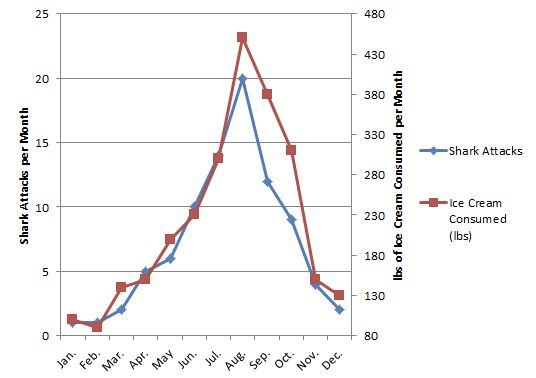
\includegraphics[width=7.44in]{images/IceCream_Shark}
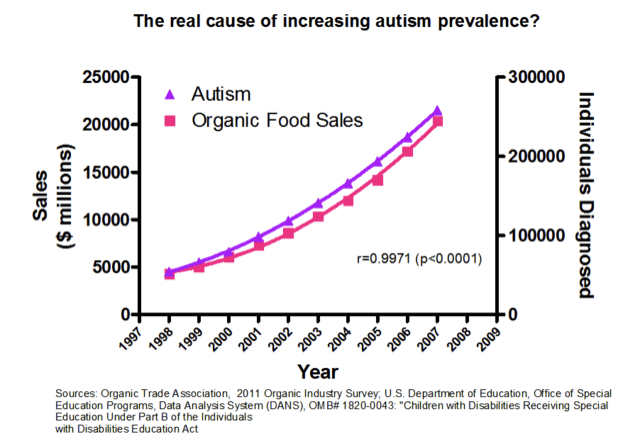
\includegraphics[width=8.89in]{images/Autism_Organic}

\hypertarget{conepts-associated-with-causation}{%
\section{Conepts associated with causation}\label{conepts-associated-with-causation}}

Mosteller and Tukey (1977) list three concepts associated with causation and state that at least two (preferably all three) are needed to support a causal relationship:

\begin{itemize}
\tightlist
\item
  \emph{Consistency} -- make a change and the response is in the same direction or the amount of response is \emph{consistent} across populations
\item
  \emph{Responsiveness} -- make a change and the response changes according to theory
\item
  \emph{Mechanism} -- make a change and we can monitor/identify a mechanism leading from cause to effect
\end{itemize}

Let's look at a classic example. Smoking and lung cancer -- from 1922 to 1947 annual deaths for lung cancer went from 612 to 9287 (Observation). This was thought in the 1950s to be either an effect of smoking tobacco or atmospheric pollution (Hypothesis). Numerous studies showed that lung cancer was more prevalent in smokers (Observation: \emph{consistency}). Chemical analyses of tobacco showed it contained carcinogens (Association: \emph{mechanism}). Public health programs resulted in a reduction in smoking and lung cancer rates decreased (Intervention: \emph{responsiveness}).

Note the initial study was an observational study and in this case it was not ethical to do the experiment per se!

\hypertarget{components-of-an-experiment}{%
\section{Components of an Experiment}\label{components-of-an-experiment}}

An experiment has \emph{treatments, experimental units, responses, and a method to assign treatments to units}. These four things specify the experimental design.

Not all experimental designs are created equal. A good experimental design must adhere to the 3Rs. It should reveal consistency, responsiveness and mechanism. The way this happens is by avoiding systematic error in measuring things, and allow estimation of error in measurements with precision.

In short, a good experimental design must:

\begin{itemize}
\tightlist
\item
  Avoid systematic error
\item
  Allow estimation of error
\item
  Be precise
\item
  Have broad validity.
\end{itemize}

Lets walk through some definitions.

If our experiment has \emph{systematic error}, then our comparisons will be biased, no matter how precise our measurements are or how many experimental units we use. \textbf{Randomisation} is our tool to combat \emph{systematic error}.

Even without \emph{systematic error}, there will be random error in the responses - this is what we call variation in what we are measuring or more formally variance. Such variation in responses invariably leads to random error in the treatment comparisons. When we compared two means in the t-test, we had to deal with the variation in both groups!

Experiments are precise when this random error in the treatment comparisons is small. Precision depends on the size of the random errors in the responses, the number of units used (\textbf{replication}), and the experimental design used.

Experiments must be designed so that we have an estimate of the size of random error. This permits statistical inference: for example, confidence intervals (which arise from standard errors) or tests of significance based on t- or F-statistics.

We cannot do inference without an estimate of this variation. We would like our conclusions to be valid for a wide population, so we need to \emph{randomise} our subjects or objects we are measuring - for example, we may need to be aware of both sexes and of young and old individuals. But there are always compromises - for example, broadening the scope of validity by using a variety of experimental units may decrease the precision of the responses.

\hypertarget{how-do-we-increase-precision-and-reduce-bias}{%
\section{How do we increase precision and reduce bias?}\label{how-do-we-increase-precision-and-reduce-bias}}

There are several key concepts

\hypertarget{blinding}{%
\subsection{Blinding}\label{blinding}}

\emph{Blinding} occurs when the evaluators of a response do not know which treatment was given to which unit. Blinding helps prevent bias in the evaluation, even unconscious bias from well-intentioned evaluators. Double blinding occurs when both the evaluators of the response and the (human subject) experimental units do not know the assignment of treatments to units. Blinding the subjects can also prevent bias, because subject responses can change when subjects have expectations for certain treatments.

\hypertarget{placebos}{%
\subsection{Placebos}\label{placebos}}

\emph{Placebo} is a null treatment that is used when the \emph{act} of applying a treatment--- any treatment --- has an effect. Placebos are often used with human subjects, because people often respond to the process of receiving any treatment: for example,
reduction in headache pain when given a sugar pill. Blinding is important when placebos are used with human subjects. Placebos are also useful for nonhuman subjects. The apparatus for spraying a field with a pesticide may compact the soil. Thus we drive the apparatus over the field, without actually spraying, as a placebo treatment.

\hypertarget{confounders}{%
\subsection{Confounders}\label{confounders}}

\emph{Confounding} occurs when the effect of one factor or treatment cannot be distinguished from that of another factor or treatment. The two factors or treatments are said to be confounded. Except in very special circumstances, confounding should be avoided. Consider the following example. We plant corn variety A in Yorkshire and corn variety B in Lancashire. In this experiment, we cannot distinguish location effects (Yorkshire vs.~Lancashire) from variety effects (cornA vs.~cornB) --- the variety factor and the location factor are confounded.

This is despite the fact that we know that Yorkshire will be better\ldots. (that's a joke)

\hypertarget{experimental-vs.-measurement-units}{%
\section{Experimental vs.~Measurement units}\label{experimental-vs.-measurement-units}}

A common source of difficulty in designing experiments is the distinction between experimental units and measurement units. We need to know the experimental units, as this is the key value used to generate our inference.

Consider an educational study, with six classrooms of 25 pupils. Each classroom of students is then assigned, at random, to one of two different reading programmes.

At the end of a six-week term, all the students are evaluated via a common reading exam.

\hypertarget{the-challenge-question}{%
\subsection{The challenge question}\label{the-challenge-question}}

\begin{quote}
Are there six experimental units (the classrooms) or 150 (25*6; the students)? We measured the reading ability of the students\ldots{} but they were in classroom sets of 25\ldots.
\end{quote}

\hypertarget{identifying-the-experimental-unit---an-example-of-pseudo-replication}{%
\subsection{\texorpdfstring{Identifying the experimental unit - an example of \textbf{pseudo-replication}}{Identifying the experimental unit - an example of pseudo-replication}}\label{identifying-the-experimental-unit---an-example-of-pseudo-replication}}

To identify the experimental units the key question is: To which \emph{thing} (students or classrooms) did we randomly allocate our treatments?

If we randomly allocated reading programmes to students, then students would be the experimental units. But we didn't, so the classroom is the experimental unit -- it is the classroom to which we randomly allocated treatments.

\emph{The classroom is the experimental unit}.

However, you are right - we don't \emph{measure} how a classroom reads; we measure how students read. Thus \emph{students are the measurement units} for this experiment.

\hypertarget{psudo-replication}{%
\subsection{Psudo-replication}\label{psudo-replication}}

Confusing these two things can lead to \textbf{pseudo-replication}. Treating measurement units as experimental usually leads to overoptimistic analysis --- we will reject null hypotheses more often than we should, and our confidence intervals will be too narrow. The usual way around this is to determine a single response for each experimental unit.

Consider an experiment with two growth chambers each containing 100 plants. One of the chambers received enhanced C02. One night after collecting data you leave the door open on the C02 chamber and the temperature drops and so the plants grow more slowly. When you come to analyze the data you get a highly significant effect of slow growth. However, that C02 results in reduced plant growth not what you expect (CO2 is good for photosynthesis\ldots).

This is an entirely plausible outcome caused by misallocating plants as the experimental unit - it was really the CO2 chamber\ldots{} to avoid such problems, one needs many chambers.

Consider a second experiment where you have 200 growth chambers and randomly allocate plants to each. If you \emph{forget to close one door} it really has no effect as just one plant is affected. In fact, to get the same effect as in the first experiment you would have to accidentally leave the doors open on all 100 of the elevated C02 chambers. This is very unlikely indeed!!!

\begin{quote}
There are 9 x 1058 ways selecting 100 chambers from 200 chambers so the chance of accidentally picking all the elevated C02 chambers is 1/ 9x10580 (stars in universe 7 x 1022).
\end{quote}

Proper \textbf{randomization} and \textbf{replication} is very different from \textbf{pseudo-replication}.

\hypertarget{randomization-properly-with-replication-protects-against-confounding}{%
\subsection{Randomization properly with Replication protects against Confounding}\label{randomization-properly-with-replication-protects-against-confounding}}

An experiment is properly randomized if the method for assigning treatments to units involves a known, well-understood probabilistic scheme. The probabilistic scheme is called a randomization.

\begin{quote}
In general, more experimental units with fewer measurement units per experimental unit works better.
\end{quote}

No matter which features of the population of experimental units are associated with our response, our randomizations should put approximately \emph{half the individuals with these features} into \emph{each treatment group}.

Recall our example above of considering sex and age of subjects and imagine a treatment with two levels (hot and cold). Done well, proper randomisation will put approximately half the males, half the females, half the older, half the younger etc into each of the treatment levels.

The beauty of randomization is that it helps prevent \emph{confounding}, even for factors that we do not know are important.

\hypertarget{haphazard-is-not-randomized---beware-the-non-randomized-experiment}{%
\subsection{\texorpdfstring{\textbf{haphazard} is NOT randomized - beware the non-randomized experiment --}{haphazard is NOT randomized - beware the non-randomized experiment --}}\label{haphazard-is-not-randomized---beware-the-non-randomized-experiment}}

A company is evaluating two different word processing packages for use by its clerical staff. Part of the evaluation is how quickly a test document can be entered correctly using the two programs. We have 20 test secretaries, and each secretary will enter the document twice, using each programme once.

Suppose that all secretaries did the evaluation in the order A first and B second. Does the second programme have an advantage because the secretary will be familiar with the document and thus enter it faster? Or maybe the second programme will be at a disadvantage because the secretary will be tired and thus slower?

Randomization generally costs little in time and trouble, but it can save us from \texttt{disaster}. The experiment above needs secretaries randomly assigned to A first -\textgreater{} B second and B first -\textgreater{} A second (50\% in each!).

Anything that might affect your responses should be \emph{randomized}! For example

\begin{itemize}
\tightlist
\item
  If the experimental units are not used simultaneously, you can (should) randomize the order in which they are used.
\item
  If the experimental units are not used at the same location, you can (should) randomize the locations at which they are used.
\item
  If you use more than one measuring instrument for determining response, you can (should) randomize which units are measured on which instruments.
\end{itemize}

\hypertarget{mini-quiz}{%
\section{Mini-Quiz}\label{mini-quiz}}

\begin{quote}
A PhD student want to determine the effects of protein on beetle reproduction, so they design an experiment with a control and protein enhanced diet. To assign beetles to each of the treatments they pour a culture onto the table and catch the first 30 beetles that run to the edge of the table, these receive the protein enhanced diet. The next 30 beetles go in the control. \textbf{Is this randomized?}
\end{quote}

(Hmm \ldots. is there anything about the first 30 beetles that reach the edge of the table that could \emph{bias} your inference?)

\hypertarget{replication-how-many}{%
\section{Replication: How many?}\label{replication-how-many}}

There is a really common question that people ask. How many replicates do I need? Unfortunatly, there are no simple rules\ldots{} it depends\ldots{} on\ldots.

\begin{itemize}
\tightlist
\item
  Resources available (\$/£/€ and equipment and time)
\item
  Variability of experimental units
\item
  Treatment structure
\item
  Size of effect (response)
\item
  Relative importance of different comparisons
\end{itemize}

There is, however, a set of tools that can help with estimating sample sizes. It's called power analysis and requires that you have some a priori estimate of the expected variation in your response variable.

\end{document}
